\documentclass[11pt,a4paper,openany]{book}
\usepackage{ctex}
\usepackage{fontenc,xunicode,xltxtra}
\usepackage{changepage}
\usepackage{amsmath,amsthm}
\usepackage{amssymb}
\usepackage{lmodern}
\usepackage{graphicx}
\usepackage{epstopdf}
\usepackage{enumerate}
\usepackage[english]{babel}
\usepackage{amsmath}
\usepackage{amssymb}
\usepackage{latexsym}
\usepackage{multirow}
\usepackage{bigdelim}
\usepackage{color}
\usepackage{graphicx}
\usepackage{wrapfig}
\usepackage{picinpar}
\usepackage{picins}
\usepackage{float}
\usepackage{clrscode}
\usepackage{algorithm} %format of the algorithm
\usepackage{algorithmic} %format of the algorithm
\usepackage{subfigure}
\usepackage{xeCJK}
\usepackage{varwidth}
\usepackage{caption}
\usepackage{lipsum}
\usepackage{framed}
\usepackage[colorlinks]{hyperref}

\setCJKmainfont[BoldFont=SimHei,ItalicFont=KaiTi]{宋体}
\setmonofont{宋体}
\setmainfont{Times New Roman}  %缺省英文字体

\XeTeXlinebreaklocale "zh"   % 针对中文进行断行
\XeTeXlinebreakskip = 0pt plus 1pt minus 0.1pt     % 给予TeX断行一定自由度
%\linespread{1.5}                                  % 1.5倍行距

\newfontfamily{\H}{SimHei}
\newfontfamily{\K}{KaiTi}
\newfontfamily{\S}{黑体}
\setCJKfamilyfont{hwxw}{STXinwei}                    %华文新魏  hwxw
\newcommand{\hwxw}{\CJKfamily{hwxw}}
\setCJKfamilyfont{hei}{SimHei}                       %黑体  hei
\newcommand{\hei}{\CJKfamily{hei}}
\setCJKfamilyfont{song}{SimSun}                      %宋体 song
\newcommand{\song}{\CJKfamily{song}}
\setCJKfamilyfont{kai}{KaiTi}                        %楷体  kai
\newcommand{\kai}{\CJKfamily{kai}}
\setCJKfamilyfont{fs}{FangSong}                      %仿宋 fsong
\newcommand{\fs}{\CJKfamily{fs}}

\newcommand{\xiaosihao}{\fontsize{12pt}{\baselineskip}\selectfont}  %字体大小
\newcommand{\wuhao}{\fontsize{10.5pt}{\baselineskip}\selectfont}

\captionsetup[figure]{name=图}
\captionsetup[table]{name=表}
\definecolor{shadecolor}{rgb}{0.92,0.92,0.92}

%\makeatletter
%\makeatother
\newtheorem{theorem}{\textbf{定理}}[section]
\newtheorem{defination}{\textbf{定义}}[section]
\newtheorem{property}{\textbf{性质}}[section]
\newtheorem{lemma}{\textbf{引理}}[section]
\newtheorem{coro}{\textbf{推论}}[section]
\newtheorem{sample}{\textbf{例}}[section]
\newtheorem{guess}{\textbf{猜想}}[section]
\renewcommand{\figurename}{图}
\floatname{algorithm}{算法}
\newcommand{\reffig}[1]{\textcolor{red}{图}\ref{#1}}

\usepackage{fancyhdr}
%\fancyhf{}
\fancyhead[LO,RE]{\leftmark}
\fancyhead[LE,RO]{cumtb.iis.ddb}
\fancyfoot[LO,RE]{}
\fancyfoot[LE,RO]{-\,\thepage\,-}
\renewcommand{\headrulewidth}{0pt}

\fancypagestyle{plain}{
     \fancyhf{}
     \fancyfoot[LO,RE]{}
     \fancyfoot[LE,RO]{-\,\thepage\,-}
     \renewcommand{\headrulewidth}{0pt}
}
\renewcommand\labelitemi{\ensuremath{\bullet}} % 原来定义为 \textbullet itemsize 黑色圆点
\usepackage{titlesec}
\titleformat{\chapter}{\centering\huge\hei}{第\,\thechapter\,章}{1em}{}[\vspace{-1cm}]
\begin{document}
\pagestyle{plain}  %取消页码
\chapter{第一章}

\chapter{第二章}
\chapter{树}
\section{树的有关定义}
\subsection{基本定义}
\begin{defination}
树的基本定义\begin{description}
        \item[树] :一个不含任何回路的连通图, 用T 表示
        \item[树枝]: T中的边,称为T 的树枝
        \item[树叶] :T 中度为一的结点
      \end{description}
\end{defination}
\begin{defination}
设e是G的一条边,若$G'=G-e$比G的连通支数增加,则称e是G的一条割边。\\
\begin{figure}[H]
  \centering
  % Requires \usepackage{graphicx}
  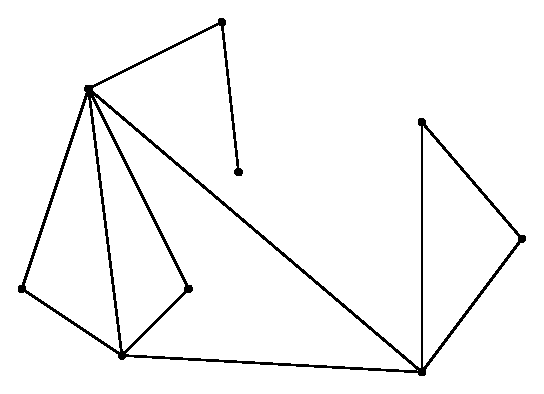
\includegraphics[width=0.7\textwidth]{3_1.eps}\\
  \caption{}
\end{figure}
\end{defination}
\begin{theorem}
$e=(u,v)$是割边,当且仅当e不属于G的任何回路。\\
\textbf{证明:}\\
\begin{itemize}
  \item 充分性(反证法):若$e=(u,v)$属于G的某个回路,则$G'=G-e$中仍存在u到v的道路,故结点u和v属于同一连通支,e不是割边。
  \item 必要性(反证法):反之,若e不是割边,则$G'$和G
的连通支数一样,因此u和v仍然处在同一个连
通支,因此在图$G'$中存在道路$P(u,v)$ $$P(u,v)+e$$就是图G的一个回路.
\end{itemize}
\end{theorem}
\begin{theorem}
$e=(u,v)$是割边,当且仅当e不属于G的任何回路。\\
\end{theorem}
\textbf{小结论:}
\begin{itemize}
  \item \textcolor{red}{树的每条边都不属于任何回路}
  \item \textcolor{red}{因此树的每条边都是割边}
  \item \textcolor{red}{树是边数最少的连通图}
\end{itemize}
\subsection{树的等价性质}
\begin{theorem}
设T 是结点数为$n\geq2 $的树, 则下列性质等价:
\begin{enumerate}
  \item T连通且无回路
  \item T 连通且每条边都是割边
  \item T连通且有n-1 条边
  \item T 有n-1 条边且无回路
  \item T的任意两结点间有唯一道路
  \item T 无回路,但在任意两结点间加上一条边后恰有一个回路
\end{enumerate}
{\hwxw 依次证明上述定理的正确性:}
{\song
\begin{itemize}
  \item (1)T连通且无回路$\Rightarrow$(2)T连通且每条边都是割边\\
  \textbf{证明:}\\
  由定理$3.1.2$ ,$e=(u,v)$是割边$\Leftrightarrow$ e 不属于G的任何回路.
  \item (2)T 连通且每条边都是割边$\Rightarrow$ (3)T 连通且有n-1 条边\\
  \textbf{证明:}\\
  采用数学归纳法: 对结点数n 进行归纳。\\
  设m(T) 为树T 的边数,n(T) 为树T 的结点数。\\
  n=2 时, 结论显然成立;\\
  设$n\leq k$ 时,$m(T)=n(T)-1$ 成立。\\
  当n=k+1 时, 由于每条边都是割边, 因此图$G'=G - e$ 有两个连通支$T_1$和$T_2$。\\
  根据假设,$$ m(T_1)=n(T_1)-1,\quad m(T_2)=n(T_2)-1 \Rightarrow m(T)=m(T_1)=m(T_2)+1=n(T)-1$$
  \item (3)T 连通且有n-1条边$\Rightarrow$(4)T 有n-1 条边且无回路 \\
  \textbf{证明:}\\
  反证法: 假定T 有回路。\\
    设C 为其中一条含有k 个结点的初级回路,故回路内有k 条边。考察C 以外的$n-k $个结点, 为保持T 的连通性, 至少需要C 以外的n-k 条
    边。所以T 的边数至少为$k+(n-k)=n$ 条与T 有$n-1$ 条边矛盾,故假设不成立,即T 无回路。
  \item(4) T有$n-1$ 条边且无回路$\Rightarrow$ (5)T 的任意两结点间有唯一道路\\
  \textbf{证明:}\\
  首先证明任意两结点间道路的存在性(反证法) : 设$u,v$ 是T 的任
意两结点, 假设不存在道路$P(u,v)$ 则$u,v$ 属于两个连通支$T_1,T_2$。 由于$m=n-1$, 则至少有一个连通支的边数不少于结点数。不妨
设为$T_1,m(T_1)\geq n(T_1)$ 设$T_1$ 无回路,由性质(1)$\Rightarrow$ 性质(2)
$\Rightarrow$性质(3),$m(T_1)=n(T_1)-1<n(T_1)$,矛盾。因此此时该连通支
$T_1$ 必存在回路, 与题目前提矛盾! 因此, $P(u,v)$ 存在。\\
其次证明任意两结点间道路的唯一性:\\
如图$3.2$, 若存在两条不同的道路$P(u,v), P'(u,v)$,则$P(u, v)\bigoplus P'(u, v)$
必存在回路。与题目假设矛盾。因此$P(u,v)$ 唯一。
\begin{figure}[H]
  \centering
  % Requires \usepackage{graphicx}
  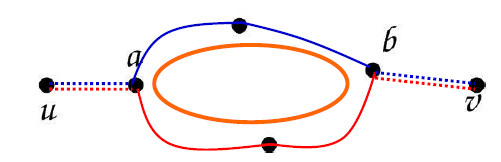
\includegraphics[width=0.6\textwidth]{3.2.png}\\
  \caption{}
\end{figure}
\item (5)T的任意两结点间有唯一道路$\Rightarrow \quad $ (6)T 无回路, 但在任意两结点间
加上一条边后恰有一个回路\\
\textbf{证明:}\\
 首先证明T 无回路:\\
若T 有回路,则回路上任意两点之间至少有两条不同的道路,与
前提矛盾。\\
故T 无回路。\\
 其次证明在任意两结点间加上一条边e 后恰有一个回路:\\
设原来两结点之间的道路为P,则$P\bigcup e $即为一个回路。\\
故在任意两结点间加上一条边e 后恰有一个回路\\

\item (6)T 无回路, 但在任意两结点间加上一条边后恰有一个回路$\Rightarrow \quad$ (1)T
连通且无回路\\
\textbf{证明:}
 T 连通:因任意两结点间加上一条边后恰有一个回路,故原图中
任意两点间必然存在一条道路。\\
T 无回路:已知条件
\end{itemize}
}
\end{theorem}
\begin{theorem}
树T中一定存在树叶结点\\
{\song
\textbf{证明:}\\
T为连通图,故不存在度为零的结点。\\
假设T中不存在树叶结点,则意味着不存在度为
1的结点,则所有结点度均不小于2。
$$ m=\frac{1}{2}\sum_{v\in V(G)} d(v)\quad \Rightarrow \quad m \geq \frac{1}{2}\cdot 2n=n > n-1$$
容易看出:矛盾!\\
}
\end{theorem}
\begin{defination}
如果T是图G的支撑子图,而且又是一棵树,则称T是G的一棵\textcolor{red}{支撑树},或称\textcolor{red}{生成树},又简称为G的\textcolor{red}{树}。
\end{defination}
\subsection{余树的概念}
\begin{defination}
G中删掉T的各边后子图称为T的\textcolor{red}{余树},记为$\bar{T}$
\end{defination}

\section{基本关联矩阵及其性质}
{\hwxw 本节研究的范围是有向连通图。}\\
\begin{defination}
有向连通图$G = (V , E)$ 的关联矩阵$B $中划去任意节点$v_k$ 所
对应的行,得到一个$(n−1)\times m$ 的矩阵$B_k$, $B_k$ 称为G 的一个基本关联矩阵。
\begin{figure}[H]
  \centering
  % Requires \usepackage{graphicx}
  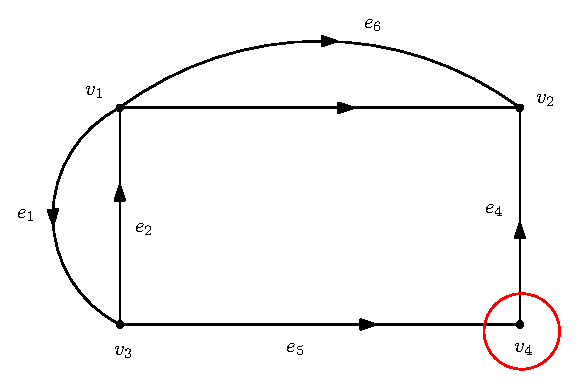
\includegraphics[width=0.6\textwidth]{3_3.eps}\\
  \caption{}
\end{figure}
\begin{equation}
B=\bordermatrix{%
       & e_1       & e_2     &e_3    &e_4  &e_5 &e_6\cr
v_1    & 1         & -1       &1     & 0 & 0 & 1\cr
v_2    & 0        & 0       &-1     & -1 & 0 & -1\cr
v_3    & -1         & 1       &0     &0 &1 &0
},
\end{equation}
\end{defination}
{\hwxw 下面我们来研究基本关联矩阵的性质。\\}
\begin{theorem}
有向图$G = (V , E)$ 关联矩阵B 的秩$ran(B) < n$。\\
{\song
\textbf{证明:}\\
关联矩阵特点:每一列都只有一个$1$和$-1$\\
n行全部相加\\
即n 个行向量线性相关,因此
$$ran B< n$$
证毕!
}
\end{theorem}
\begin{theorem}
设$B_0$是有向图G关联矩阵B的任意一k阶子方阵,则$det(B_0)$为$0,1$或$-1$\\
{\song
\textbf{证明:}\\
若$B_0$某列全零,则$det(B_0)=0$\\
若$B_0$每列都有两个非零元,则$det(B_0)=0$\\
若$B_0$存在某列只有一个非零元,则按该列展开可知$det(B_0)=\pm det(B_1)$\\
依次类推,可证!
}
\end{theorem}

\begin{theorem}
设$B_0$是有向图G关联矩阵B的任意一k阶子方阵,则$det(B_0)$为$0,1$或$-1$\\
{\song
\textbf{证明:}\\
若$B_0$某列全零,则$det(B_0)=0$\\
若$B_0$每列都有两个非零元,则$det(B_0)=0$\\
若$B_0$存在某列只有一个非零元,则按该列展开可知$det(B_0)=\pm det(B_1)$\\
依次类推,可证!
}
\end{theorem}

\begin{theorem}
设B是有向连通图G的关联矩阵,则$$ran B=n-1$$
{\song
\textbf{证明:}\\
设B中最少的线性相关行数为$l$\\
则$l\leq n$,其对应图中结点$v(i_1),v(i_2),\dots,v(i_l )$\\
\begin{equation*}
k_1\cdot b(i_1) +k_2\cdot b(i_2) +\cdots +k_l\cdot b(i_l) =O_m \quad (k_j\neq 0,\quad j=1,2,\cdots,l)
\end{equation*}
\begin{itemize}
  \item
  \begin{center}
    所有$b(i_j)$中,第$t(t=1,2,\cdots m)$个分量可能
  \end{center}
  \item
  \begin{center}
    所有$b(i_j)$中,第$t(t=1,2,\cdots m)$个分量可能
  \end{center}
  \item
  \begin{center}
    所有$b(i_j)$中,第$t(t=1,2,\cdots m)$个分量不可能
  \end{center}
\end{itemize}
  \begin{flushleft}
    否则,该分量最终不可能为$0$。
\end{flushleft}
\quad 这样,我们可以对矩阵B进行行、列交换,使前$l$行为线性相关的各行\\
\quad 再针对这$l$ 行中,有两个非零元的列换到前$r$列\\
则此$l$ 行中,其余$(m-r)$列将均为零元\\
\quad 此时矩阵B将变为
\begin{align*}
 B'= \begin{array}{lc}
\mbox{}&
\begin{array}{cc}r&m-r \end{array}\\
\begin{array}{c}l\\n-l\end{array}&
\left[\begin{array}{cc}
P&0\\
0&Q
\end{array}\right]
\end{array}
\quad \quad ran B=ran B'
\end{align*}
\quad 若$l <n$,则从$B'$可清楚看出,图G为两个连通支,这与
图G为连通图矛盾!\\
因此,一定有$l=n$
}
\end{theorem}

\end{document}
